\documentclass[9pt, a4, twoside]{article}
\usepackage[utf8]{inputenc}
\usepackage[]{authblk}
\usepackage{amsmath}
\usepackage{hyperref}
\usepackage[in]{fullpage}
\usepackage{graphicx}

\title{Testing of a stochastic fluctuation of the speed of light: the REWOLF project}
%\author{Christophe M.F. Hugon\thanks{funded by the ShareLaTeX team}, Antonio Orzelli\thanks{funded by the ShareLaTeX team}, Vladimir Kulikovskyi}

\author[1]{Principal investigator: Christophe M.F. Hugon}
\author[2]{Second investigator: Vladimir Kulikovskiy}
\author[1]{Antonio Orzelli}

\affil[1]{INFN, Sezione di Genova}
\affil[2]{INFN, Laboratori Nazionali del Sud}

\date{August 2014}

\begin{document}

%\begin{titlepage}
\maketitle
\begin{abstract}
In this proposal, we show that by using standard instrumentation we can measure a possible fluctuation of the group velocity of light as predicted by some theories. We also introduce the idea to integrate this apparatus in an existing long baseline experiment to reach the finest results.
\end{abstract}

\section{Scientific background}

The speed of light can be decomposed in three components:
\begin {itemize}
\item The first is defined as the maximum speed, and leads to the Special Relativity. This speed ($c_{rel}$) appears in the Lorentz transformation and is the one that defines the relationship between the mass and the energy,
\item The second is the magnetic wave speed, which is commonly called phase velocity ($c_{\Phi}$),
\item Finally, the speed of a photon propagation (in the quantic mean of momentum). It is called the group velocity ($c_{group}$), and is defined in average as $c_{group}=L/T$ where $L$ is the distance traveled and $T$ the transit time through $L$.
\end {itemize}
While $c_{rel}$ is not expected to fluctuate and is strongly tested, some theories predict that $c_{\Phi}$ and $c_{group}$ can fluctuate during the propagation in vacuum.

~

In the considered theories, a fluctuation is expected to be stochastic and can be studied with the arrival time of a short light pulse after propagation in the vacuum. The longer the propagation path, the wider the timing enlargement of the pulse is.

In the first family of theories (Th 1), the group velocity fluctuations are predicted if the photon propagation is considered as a succession of interactions with pairs of ephemeral (virtual) fermions. This kind of model is developed in \cite{baseTh} and independantly  in \cite{baseTh2}. More generally, from such definition of the vacuum filled with virtual fermions, one can demonstrate that the values of the parameters $\mu_0$ and $\epsilon_0$ and the group speed of light appear naturally at the correct scale. Moreover, the equation $\langle c_{group}\rangle  = c_{Phi} = \sqrt{1/(\mu_0\epsilon_0)}$ where $\langle c_{group}\rangle$ is the mean value of the group velocity, can be deduced independently of the Maxwell equations.

This description of the vacuum predicts fluctuations of the photons' transit time of the order of
\begin{displaymath}
\sigma_t(\mathrm{FWHM}) \approx 120\times10^{-15}\mathrm{s}\cdot L^{-1/2}
\end{displaymath}
at the distance $L$. The experimental signature of such an effect is an enlargement of the light pulse temporal envelop during its propagation. This enlargement increases proportionally to the square root of the path length in the vacuum.

There are two elements to note in this model. First, the lifetime of the virtual pair is inversely proportional to the square root of the total pair energy. This order of magnitude of 120 is given for a peaked energy distribution, considering averaged parameters instead of their full distribution (as lifetime of pairs, Heisenberg principle\ldots). The second one is that since no final interpretation is given to this energy distribution, its average can be bigger (with weak effect on the fluctuations' order of magnitude), or smaller (a non relativistic level of energy bring the fluctuation FWHM at $\sigma_t \approx 240\times10^{-15}\mathrm{s}\cdot L^{-1/2} $.

In this model, this phenomenon is totally independent of the light wavelength and the phase as it relies only on a photon interaction probability with the ephemeral pairs.

In the second family of theories (Th 2), the effects are at smaller scale, but for some of them and under certain conditions, they are reachable in our proposed experiment. These theories are based on physics beyond the standard model, like Quantum Gravity \cite{gravcite} and have a sensibly different behaviour as a function of distance and energy.
Assuming additional dimensions, the Quantum Gravity theory implies a dispersion in function of distance of $[\mathrm{s}]/[\mathrm{m}]^\mathrm{n}$ where $\mathrm{n} \geq 1$. If a speed of light fluctuation is detected, it is essential to measure its spread at different distances to differentiate the theories. Note that in these theories we can have a velocity fluctuation dependency on energy, which makes doing a spectral measurement of the arriving pulse interesting.

There is a third family of theories (Th 3) concerning space/time fluctuations at Planck scale. This implies a too small scale to be detected by the proposed method, or the effect impacts also the phase speed which can be measured much more precisely thanks to interferometry \cite{th3}.
It is important to note that for any model that implies a space/time fluctuation as an effect on $c_{Phi}$ and $c_{group}$ at the same scale, an interferometry system is more adapted, due to its very accurate precision.

\section{State of art}


%Currently, only one other collaboration work on such a reasearch in collaboration with the Celia laboratory\footnote{http://www.celia.u-bordeaux1.fr/spip.php?article435}.
Presently, this research is carried on by the FLOWER collaboration, jointly with the Celia laboratory\footnote{\url{http://www.celia.u-bordeaux1.fr/spip.php?article435}}.
The current limit put on this fluctuation effect is $\sigma_t(\mathrm{FWHM}) \approx 700 \times 10^{-15}s.m^{-1/2}$ \cite{cosmoobs}.

The purpose of this project is to push this limit down to the theoretical predictions, and possibily, to distinguish different predicted fluctuations, and principally from the Th 1.

In the case of $100~\mathrm{m}$ light path and $2~\mathrm{fs}$ detector sensitivity the current cosmological limit can be reached in laboratory.

\section{Objectives of the proposal}

The objective of the REWOLF project is to detect a possible group velocity fluctuation of light in a vacuum, larger than a possible phase velocity fluctuation. It is important to note that even if a limit based on cosmological observations was put, no dedicated experiment has yet reached the predictions from recent theoretical models.

The final goal of this experiment is to use ultrashort pulses of $5~\mathrm{fs}$ FWHM and a path of $1$ to $10~\mathrm{km}$. According to the predictions of the foregoing first family of theory, the time width of the pulse is expected to be spread to $9~\mathrm{fs}$ (FWHM). It is possible to see this enlargement using detectors with a resolution of about $2~\mathrm{fs}$.

The best method to characterize both the initial and final pulses must be an intensity auto-correlation system. This type of detector is described in the section \ref{sec:detector}
The next parts present a description of the different phases of the experiment and the suggested technical solutions.

\section{Description of the proposed research activity and milestones}

The setup has three main components: the light sources, the propagation path and the detector. We plan several phases of the experiment:
\begin{itemize}
\item[Phase-0)] 6 months: Laboratory tests of the source and the detector. During this phase, the source's properties and the accuracy of the detector are validated.
\item[Phase-1)] 8 months: Laboratory measurements with a multi-reflections cell \cite{herriottcell}. In this phase we plan to reach the current cosmological limit of the light transit time fluctuations. The light path should reach the 100 m scale. It was calculated that an accurate measurement can overtake this limit by about 30\% (fig. \ref{fig:sensiv}).
\item[Phase-2)] 10 months: Using the knowledge out of the phase-0 and phase-1 (source, mirrors and detector), the final experimental setup will use a km-scale path. Here we plan to reach the model limit for the light transit dispersion. In this proposal we want to investigate two possibilities: an improved Herriot cell, or to integrate the setup with a long baseline detector. In Italy, a very good candidate could be the \textsc{virgo} facilities \footnote{\url{https://wwwcascina.virgo.infn.it/}}.
\end{itemize}
The research for a future integration in a long baseline detector will be under preparation and discussion during the full developpement process. This element is for us a very important point, because, for a better sensitivity, such an integration would strengthen the longevity of the experiment.

In the next sections, the technical solutions of the experiment components are described.

\subsection{Source}

In  the modern ultrashort pulse applications, the Titanium-Sapphire lasers are used thanks to the simple handling compared to the previously used dye lasers. Ti-Sapphire lasers are able to produce pulses with a width  below $10~\mathrm{fs}$. The typical pulse energy is $2-6~\mathrm{nJ}$ and the rate is about $80~\mathrm{MHz}$. The wavelength has a range of about $700-1000~\mathrm{nm}$\footnote{Rainbow oscillator \url{www.femtolasers.com}, Octavius-85 \url{www.thorlabs.de}}. The  divergence  is $<2~\mathrm{mrad}$ and the beam diameter is $< 2.5~\mathrm{mm}$. For the pulse measurement an energy of several nJ may not be enough. In this case an  amplification should be used. A Ti:Sapphire multipass amplifier with the dispersion compensation is able to provide $<25~\mathrm{fs}$ pulses with energy  of $\approx1~\mathrm{mJ}$, but reduces the pulse rate to the kHz scale, keeping the divergence $<2~\mathrm{mrad}$  and increasing the beam diameter to $15~\mathrm{mm}$. Stretching this pulses is possible to $<7~\mathrm{fs}$ with hollow  fiber compressors. \footnote{The data are taken for CEP Pro amplifier + Kaleidoscope compressor \url{www.femtolasers.com}}. The state of art for the compression is $4~\mathrm{fs}$ from the amplificator. At this order of magnitude the measurement method gives the real limitation on the time resolution. \footnote{MOSAIC OS compressor\\ \url{http://pdf.directindustry.com/pdf/femtolasers-produktions-gmbh/mosaic-os-octave-spanning-gdd-module/36035-231646.html}}

\subsection{Light path}

Considering the phase-1 of the proposal we need a Herriott cell at meter scale with about 100 reflections on mirrors. To ensure $< 2/3$ energy loss at the end of the path, $>0.99$ reflectivity coefficient is required. This requirement is possible with gold mirrors with a roughness of less than 100 Å. The state of art is the 1 Å scale  \footnote{\url{http://www.thorlabs.de/NewGroupPage9.cfm?objectgroup_id=7028}}. This kind of mirrors are commercially available. The time dispersion due to thermal fluctuations of the mirrors are expected to be negligible compared to the dispersion due to the mirror roughness, but it should be tested in the phase-0.

The air group velocity dispersion is of the order of $1~\mathrm{fs}^2/\mathrm{m}$ (at 1 atm) \cite{airdispertion} Which represents, for a pulse of $5~\mathrm{fs}$ width, a dispersion of $0.2~\mathrm{fs}/\mathrm{m}$. This dispersion is directly proportional to the pressure. That means that to reach a negligible total dispersion (less than $10\cdot10^{-15}\mathrm{s}$), the pressure should be less that $0.5~\mathrm{mbar}$ for the $100~\mathrm{m}$ scale experiment, and less than $0.05~\mathrm{mbar}$ for the km scale. These orders of magnitude are quite easy to reach in both cases.

According to the experience from the phase-1, the extension to the phase-2 is straightforward. Due to the length of several kilometers, $0.1~\mu\mathrm{rad}$ divergence of the light source is needed to keep a cm scale beam radius. This constraint will require an additional optical collimator.

Note that in the case of the integration in a long baseline experiment like \textsc{virgo}, the pressure inside the detector is very low ($10^{-11}~\mathrm{mbar}$ for \textsc{virgo}), and is far better than the requirements for the proposed experiment.
Moreover, the  use of such a facility would strongly reduce the number of reflections, which will decrease the systematic errors sources and the overall complexity.

For a long baseline detector, a dedicated study will be required to determine the compatibility of our detector setup with the facility. First contact with the \textsc{virgo} collaboration was made, and members in our Institute will help clarifing this part.

\subsection{Detector}
\label{sec:detector}
For this experiment, a direct spectrometry or phase measurement method cannot be used, because they rely on some assumptions about the pulse properties and use the Fourier limit to deduce its shape.

%On the other hand comes after on the one hand...
On the other hand an autocorrelation system is based on the effective interaction of the photon with a cristal, which allows to determine precisely the electric field of the pulse without any assumptions.

For this alternative, there are several kinds of autocorrelator detectors, and FROG \cite{frogref} (Frequency Resolved Optical Gating) which satisfies the requirements.

\begin{figure}[!]
\centering
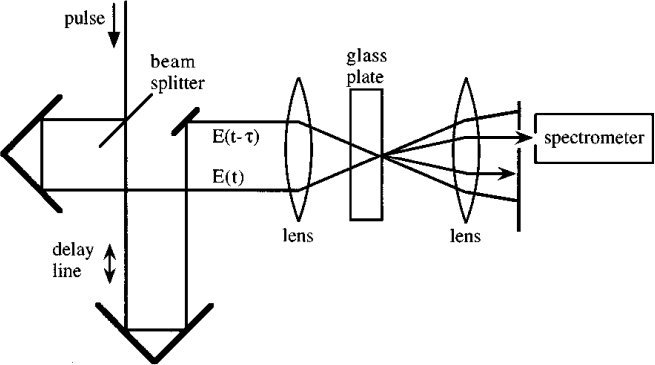
\includegraphics[width=0.5\textwidth]{./img/thg_setup.png}
\caption{FROG system scheme. The pulse is split, one component is delayed. A beam is produced by harmonic generation autocorrelation in a crystal. The generated beam is detected by a spectrometer.}
\label{fig:sensiv}
\end{figure}

In general the measurement is done by splitting the pulse beam in two parts and sending them on a non-linear crystal. The crystal, thanks to the second or third harmonic generation effect, will produce an output beam proportional to the cumulative intensity of the input beams. By adding a delay to one of the incoming beam (changing one path length), it becomes possible to measure the full autocorrelation of the incoming pulse.

By using a surface third harmonic generation FROG it is possible to characterize pulses with $\approx5~\mathrm{fs}$ width and an intensity of few nJ. The time resolution of such a system can reach the sub fs order of magnitude ($0.2~\mathrm{fs}$).

\section{Perspectives, conclusions and scientific impact}

\begin{figure}[!]
\centering
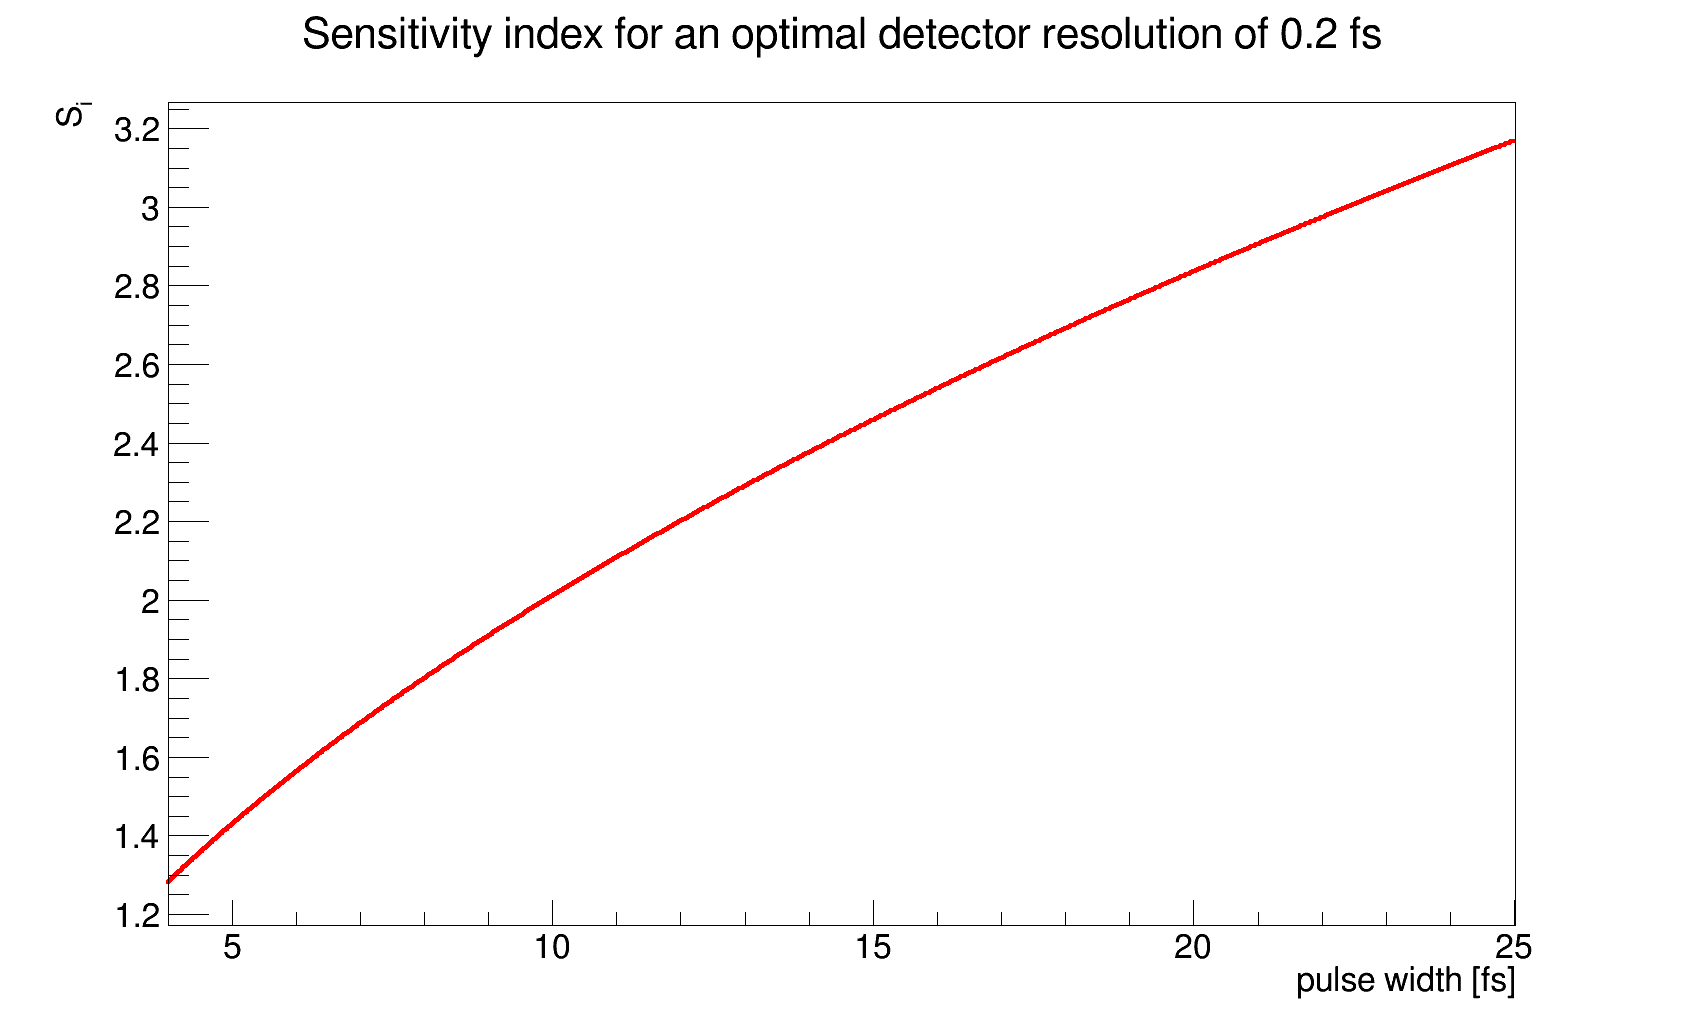
\includegraphics[width=0.70\textwidth]{./img/Pwdependency.png}
\caption{Sensitivity index for a resolution of $0.2~\mathrm{fs}$ in function of the laser pulse width.}
\label{fig:sensivindex}
\end{figure}

\begin{figure}[!]
\centering
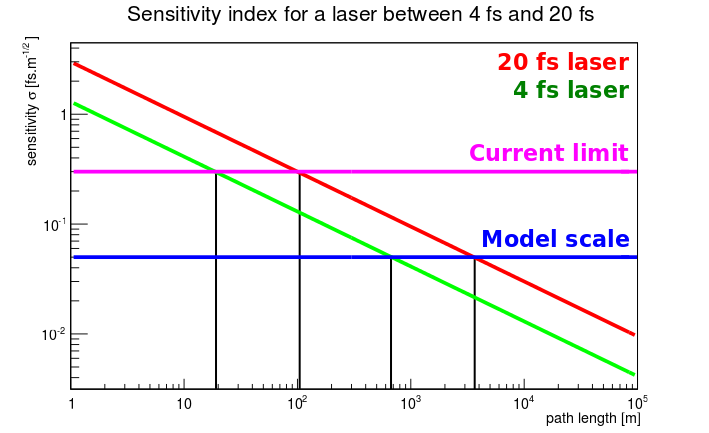
\includegraphics[width=0.7\textwidth]{./img/total_sensitivity.png}
\caption{Sensitivity for different cases of laser pulse width (detector resolution of $0.2~\mathrm{fs}$). The current limit is given by cosmological analysis, the Model scale is for the model order of magnitude defined in the Th. 1.}
\label{fig:sensiv}
\end{figure}

If we consider a light pulse as a gaussian photon distribution, the sensitivity index of this experiment can be calculated by

%%%%PLEASE, WHEN ARE WE, IN 1995?
\begin{displaymath}
S_i = \sqrt{(R+P_W)^2-P_W^2}\quad,
\end{displaymath}
where $R$ is the total resolution of the experiment, and $P_W$ the pulse width. This allows to get the total sensitivity $S$:
\begin{displaymath}
S=S_i/\sqrt{L}
\end{displaymath}

Given that the FROG sensitivity is not the heaviest part in the total cost, we consider now that the privileged solution is a $0.2~\mathrm{fs}$ resolution. It permits to evaluate the sensitivity index, represented in the figure \ref{fig:sensivindex} and the total sensitivity, represented in the figure \ref{fig:sensiv}.

Therefore we can set the goals of the experiment:

In the most pessimistic solution for the laser, we can push back the current limit with a $100~\mathrm{m}$ path and the detection of the fluctuations are allowed for about $3~\mathrm{km}$ to $6~\mathrm{km}$. We could exclude the fluctuation hypothesis at $3\sigma$ with a path of $4~\mathrm{km}$ and a path of $10~\mathrm{km}$ can exclude it at $5\sigma$ (considering a fluctuation of $50 \cdot10^{-15}\mathrm{s}.\mathrm{m}^{-1/2}$).

    %the measurement at 6 km can exclude no fluctuation hypothesis at 3 sigma, assuming the 50 as/m1/2 fluctuation. The additional measurement at 12 km can exclude no fluctuation hypothesis at 5 sigma.

In the case of a fluctuation measurement, to exclude the linear dependance of the fluctuations with distance (instead a square root dependance, $S=S_i/L$), which is expected in some alternative models (although at smaller scale) 18 km measurement (equivalent to 3 round trips in the \textsc{virgo} tunnel) is enough to reach $5\sigma$ difference. %%TOO MANY () IN THIS PHRASE FIXME !!!

In the most optimistic case of a laser of $4~\mathrm{fs}$, we could push back the current limit at the 10 meter scale (easy to reach in phase-1), and gain one order of magnitude for the fluctuation hypothesis detection or exclusion.

Therefore  it is clear that this research program is very ambitious. Even if it uses common and well known technologies (almost all of the material is commercially available for industrial uses), it will need a good experimental mastery and a excellent artifact control and analysis.

Nevertheless, for us, these skills seem to be reachable. The team that we are forming combine a theoritical knowledge, a reliable experimental experience and a steady electronics/DAQ. We are convinced that, thanks to such an experiment, we will be able either to detect a group velocity  fluctuation, or to set a new strong limit that confirms that the group velocity and the phase velocity are indifferentiable at a scale of the attosecond per square meter (and much further for a direct  proportionality with the distance). In any case this result will be very interesting for the physics community, so we wish to get the opportunity offered by your funding proposal to perform this experiment.



\begin{thebibliography}{9}

 \bibitem {baseTh}
 M. Urban, F. Couchot, X Sarazin, A. Djannati-Atai, Eur. Phys. J. D (2013) 67: 58


 \bibitem {baseTh2}
 Appl. Phys. B 100, 9 (2010)

\bibitem {gravcite}
 H. Yu, L.H. Ford, Phys. Lett. B 496, 107 (2000)

 \bibitem {th3}
 C.J. Hogan, FERMILAB-PUB-10-036-A-T, arXiv:1002.4880v27

 \bibitem {cosmoobs}
 A.A. Abdo et al., Nature 462, 331 (2009)

 \bibitem {herriottcell}
 Applied Optics, Vol. 46, Issue 22, pp. 5408-5418 (2007)

 \bibitem {airdispertion}
 P. J. Wrzesinski and all, Optics Express, Vol. 19, Issue 6, pp. 5163-5170 (2011)

 \bibitem {frogref}
 R. DeLong and all, Review of Scientific Instruments, 68, 3277-3295 (1997)

\end{thebibliography}

\end {document}
